\documentclass[12pt,answers]{exam}

\usepackage{amsmath,amsfonts,amssymb,mathtools,physics,commath}
\usepackage{todonotes}
\usepackage{float}
\usepackage{multicol}
\usepackage{polynom}
\usepackage{siunitx}

\newcommand{\inv}{^{-1}}

\pagestyle{headandfoot}
\firstpageheadrule
\runningheadrule
\firstpageheader{Math 221}{Exam 2|Solutions, Page \thepage\ of \numpages}{March 5, 2019}
\runningheader{Math 221}{Exam 2|Solutions, Page \thepage\ of \numpages}{March 5, 2019}
\runningfooter{}{}{}

\begin{document}
% \maketitle
\begin{questions}

\question
Evaluate the following integrals.
\begin{parts}
    \part[10]
    $\displaystyle \int \frac{3x^2+2x+13}{x^2+4} \dif x$
    \begin{solution}
        Long division gives
        \[
            \polylongdiv{3x^2+2x+13}{x^2+4}
        \]
        so
        \begin{align*}
            \int \frac{3x^2+2x+13}{x^2+4} \dif x
             & = \int \left( 3 + \frac{2x+1}{x^2+4} \right) \dif x               \\
             & = 3x + \int \frac{2x}{x^2+4} \dif x + \int \frac{1}{x^2+4} \dif x \\
             & = \boxed{3x + \ln(x^2+4) + \frac12 \tan[-1](\frac x2) + C}
        \end{align*}
    \end{solution}
    \part[12]
    $\displaystyle \int \frac{2x^2-5x-1}{x^3-x} \dif x$
    \begin{solution}
        Partial Fractions:
        \[
            \frac{2x^2-5x-1}{x(x-1)(x+1)} = \frac{A}{x} + \frac{B}{x-1} + \frac{C}{x+1}
        \]
        Clearing denominators:
        \[
            2x^2-5x-1 = A(x-1)(x+1) + Bx(x+1) + Cx(x-1)
        \]
        Solving gives $A = 1$, $B = -2$, $C = 3$.
        Hence
        \begin{align*}
            \int \frac{2x^2-5x-1}{x^3-x} \dif x
             & = \int \left( \frac 1x + \frac{-2}{x-1} + \frac{3}{x+1}\right) \\
             & = \boxed{\ln|x| -2 \ln|x-1| + 3 \ln|x+1| + C}
        \end{align*}
    \end{solution}
\end{parts}

\newpage
\question
\begin{figure}[H]
    \centering
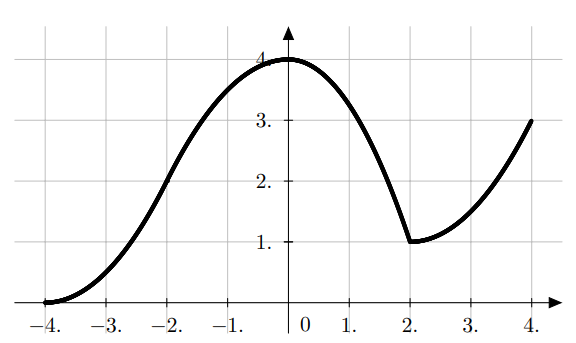
\includegraphics[width=.4\textwidth]{graphics/2019-spring-exam2-2.png}
\end{figure}
For the function $y = f(x)$ graphed above, approximate the definite integral $\int_{-4}^4 f(x) \dif x$ using
\begin{parts}
	\part[6]
    The Trapezoidal rule for $T_4$.
	\begin{solution}
        $\Delta x = \frac{4-(-4)}{4} = 2$
        \begin{align*}
            T_4 
            &= \frac{\Delta x}{2} \left(f(-4) + 2 f(-2) + 2 f(0) + 2 f(2) + f(4)\right) \\ 
            &= 1 \left( 0 + 2(2) + 2(4) + 2(1) + 3\right) = \boxed{17}
        \end{align*}
	\end{solution}
	\part[6]
	Simpson's rule for $S_4$.
	\begin{solution}
       Again,  
        $\Delta x = \frac{4-(-4)}{4} = 2$.
        \begin{align*}
            S_4 
            &= \frac{\Delta x}{3} \left(f(-4) + 4 f(-2) + 2 f(0) + 4 f(2) + f(4)\right) \\ 
            &= \frac{2}{3} \left( 0 + 4(2) + 2(4) + 4(1) + 3\right) = \boxed{\frac{46}{3}}
        \end{align*}
	\end{solution}
\end{parts}

% \newpage
\question[6]
Give the partial fraction expansion of the rational function using coefficients $A, B, C, \ldots$, but \textbf{do not} solve the values of the coefficients.
\[
    f(x) = \frac{2x^4 - 5x + 3}{(x^2+2x+1)(x^2+x+1)^2}
\]
\begin{solution}
    Notice that $x^2+2x+1 = (x+1)^2$, whereas $x^2+x+1$ is irreducible, so
    the partial fraction expansion is of the form
    \[
        \frac{A}{x+1} + \frac{B}{(x+1)^2} + \frac{Cx+D}{x^2+x+1} + \frac{Ex+F}{(x^2+x+1)^2}
    \]
\end{solution}

\newpage
\question 
Evaluate the integrals using proper limit notation.
\begin{parts}
	\part[8]
	$\displaystyle \int_0^\infty x e^{-x} \dif x$
	\begin{solution}
        \begin{align*}
            &\lim_{b\to\infty} \int_0^b x e^{-x} \dif x
            \qquad \qquad
            \begin{array}{ccc}
                & D & I \\ 
                + & x & e^{-x} \\ 
                - & 1 & -e^{-x} \\ 
                + & 0 & e^{-x} \\ 
            \end{array}
            \\
            &= \lim_{b\to\infty} \left[ -xe^{-x} - e^{-x} \right]_0^b \\ 
            &= \lim_{b\to\infty} \left[ -be^{-b} - e^{-b} - (-1) \right] \\ 
            &= \lim_{b\to\infty} \frac{-b-1}{e^b} + 1 \\ 
            &\overset{LH}{=} \lim_{b\to\infty} \frac{-1}{e^b} + 1
            = \boxed{1}
        \end{align*}
	\end{solution}
	% \newpage
	\part[8]
	$\displaystyle \int_{2}^6 \frac{1}{\sqrt{6-x}} \dif x$
	\begin{solution}
        \begin{align*}
            \lim_{b\to6^-} \int_2^b \frac{1}{\sqrt{6-x}} \dif x 
            & = \lim_{b\to6^-} \left[ \eval{-2\sqrt{6-x}}_2^b \right] \\ 
            & = -2 \lim_{b\to6^-} \left( \sqrt{6-b} - \sqrt{4} \right) \\ 
            & = -2 (0 - 2) = \boxed{4}
        \end{align*}
	\end{solution}
\end{parts}

% \newpage
\question[8]
A spring requires a force of 2 newtons to stretch it 1 meter beyond its rest length. How much work is required to stretch the spring from 1 meter to 3 meters beyond its rest length?
\begin{solution}
    The first sentence allows us to compute the spring constant:
\[
    F =  kx \implies 2= k(1) \implies k = 2
\]
Then
\[
    W 
    = \int_1^3 2 x \dif x 
    = \eval{x^2}_1^3 = 9-1 = \boxed{8 \text{ Joules}} 
\]
\end{solution}

\newpage
\question
\begin{parts}
    \part[8]
    Find the arc length of the curve $y = x^3$, $0 \le x \le 1$.
    Just set up the integral. \textbf{Do not evaluate.}
    \begin{solution}
        \[
            L = \int_0^1 \sqrt{1+(3x^2)^2} \dif x
            = \boxed{\int_0^1 \sqrt{1+9x^4} \dif x}
        \]
    \end{solution}
    \part[10]
    Find the surface area of the surface generated by rotating the curve in part (a) around the $x$-axis. \textbf{Evaluate the integral.}
    \begin{solution}
        \begin{align*}
            SA 
            &= \int_0^1 2\pi x^3 \sqrt{1+9x^4} \dif x & (u=1+9x^4; \dif u = 36x^3 \dif x) \\
            &= \frac{\pi}{18} \int_1^{10} \sqrt{u} \dif u \\
            &= \frac{\pi}{18} \cdot \frac23 \left[ u^{3/2}\right]_1^{10} \\
            &= \boxed{\frac{\pi}{27}(10^{3/2} - 1)}
        \end{align*}
    \end{solution}
\end{parts}

\newpage
\question[10]
A cylindrical tank of radius 5 ft and height 10 ft is filled with water of density $\rho\ \unit{lb/ft^3}$. How much work is required to pump all of the water out of the top of the tank? Set up and evaluate an appropriate integral.
\begin{solution}
    Let $x$ denote the distance to the top of the tank.
    The force to move a slice of water of width $\Delta x$ is $F = ma = \rho V = \rho \pi r^2 h = \rho \pi 25 \Delta x$. 
    Work is then
    \[
        W = \int_0^{10} \rho 25 \pi x \dif x
        = \rho 25 \pi \int_0^{10} x \dif x
        = \rho 25 \pi \left[\frac{x^2}{2} \right]_0^{10}
        = \boxed{\rho 1250 \pi \ \unit{ft.lbs}}
    \]
\end{solution}

\question[10]
Find the centroid $(\overline x, \overline y)$ of the region bounded by the semicircle $y = \sqrt{9-x^2}$, $-3 \le x \le 3$ and the $x$-axis.
(You may use symmetry and the area formula for a circle.)
\begin{solution}
    By symmetry of the region, $\overline x = 0$.
    To compute $\overline y$:
    \begin{align*}
        m &= \int_{-3}^3 \sqrt{9-x^2} 
        = \frac12 \pi \cdot 9 
        = \frac92 \pi & (\text{formula for area of semicircle}) \\ 
        M_x &= \frac12 \int_{-3}^3 (9-x^2) \dif x & (\text{symmetry of even functions})\\
        &= \frac 12 \cdot 2 \int_0^3 (9-x^2) \dif x \\
        &= \eval{9x - \frac{x^3}{3}}_0^3 
        = (27 - 9) - 0 
        = 18
        \\ 
        \overline y &= \frac{M_x}{m} = 18 \cdot \frac{2}{9\pi} = \frac{4}{\pi}
    \end{align*}
    Thus the centroid is $\boxed{(0, \tfrac4\pi)}$.
\end{solution}
\end{questions}
\end{document}
